\chapter{Concepts}
Shark is a peer-to-peer (P2P) system. To avoid any misconceptions, we have to define our understanding of the term {\it peer} first.

\begin{itemize}
\item
A peer is meant to be a piece of software that runs on some hardware.

\item
Each Shark peer has an {\it owner} which is either a person or a group of persons. A group is constituted by a number (greater than one) of persons and other groups. A group may solely consists of persons, but a group is allowed to contain both: Persons and other groups.

{\it Owning} means that the person/group has full access rights to the software.
A peer derives its identity from its owner. A peer has only one owner, but a owner is allowed to own multiple peers.

\item
A peer contains data. Its owner has full access to this data. Shark offers no concepts to protect data from owners. Nevertheless, application developers can decide to encrypt data but this is out of scope of the framework itself.

\item
Peers can communicate with other peers. Shark has its own communication protocol (KEP) which will be explained briefly later. This protocol defines two messages types. It does not define what a peer has to do after receiving a message.

\item
Peers can communicate via arbitrary protocols. The Shark protocol KEP is stateless and message-oriented which has implications: Peers cannot assume that sent messages reach their recipients. Applications are free to implement hand-shake protocols on top of KEP, though.

Peers cannot assume to meet other peers again. Such weak assumptions on communication protocols make it possible to run Shark application even in spontaneous networks like Bluetooth networks, ad-hoc mode W-LAN networks etc. Shark does not even require Internet. It can work on any protocol that is (sometimes) capable of transmitting data, see section \ref{ref:sec:KEP}.

\item
Communication can be encrypted and signed, see section \ref{sec:security}.

\item
Each peer can store arbitrary information in a {\it Shark Knowledge Base (SharkKB)}, section \ref{sec:sharkkb}.


\end{itemize}

A first sketch may illustrate the mayor concepts, see \ref{fig:generalConcept}.

\begin{figure}[t]
\centering
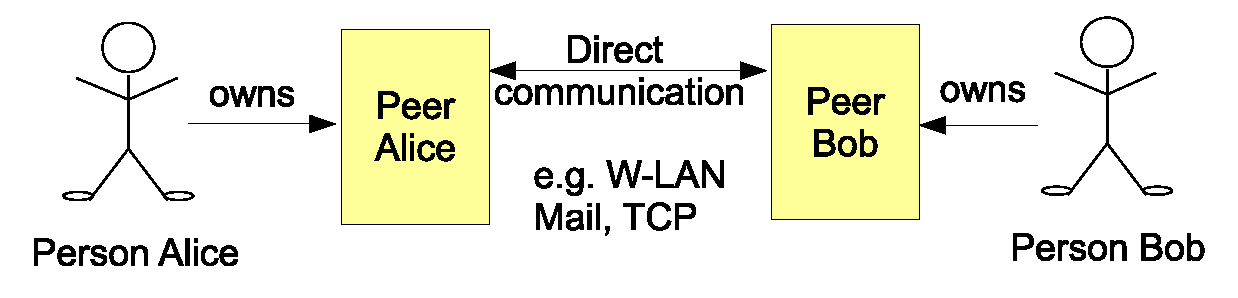
\includegraphics[width=0.60\textwidth]{generalConcept.eps}
\caption{People own peers which can communicate}
\label{fig:generalConcept}
\end{figure}

\section{Communication principles}
The Shark communication protocol is called {\it Knowledge Exchange Protocol (KEP)}. It has just two message types:

\begin{description}
    \item[Expose (interest)]
Owners can define their {\it interests}. One might define that he is interested in {\it cooking, skiing} and {\it Star Trek}\footnote{which was a TV series in the 1990th in the US which the author liked (and still likes) very much.} Another one might be interested in {\it vegetarian cuisine, sports} and {\it science fiction}.

At the first syntactical glance, both peers don't have anything in common. Sports isn't the same as skiing and vegetarian food isn't just food. A bit more elaborated semantic view can reveal that skiing is a {\it kind of} sport etc., though.

Shark provides a semantic data model which helps to recognize that both peers have similar interest. This point will be explained later in more detail.

Moreover, a peer can define with whom it is interested in communicating, what time and at which place. But most importantly a peer is able to define if s/he wants to sent or/and receive information to/from a particular peer.

    \item[Insert (knowledge)]
Knowledge is constituted of information. Each information is put into a {\it context}. A context describes aspects of information, namely information topic, issuer, location and time. Peers can exchange such contextualized information at any time. Peers can received knowledge at any time. And they can do with it whatever they like.
\end{description}

KEP is an {\bf asynchronous protocol} which means that a peer doesn't have to wait for a reply. Each peer can send a message whenever it likes, e.g. when meeting another peer. A peer cannot expect a reply: The other peer might not like to answer or the communication channel is broken during communication.

\subsection{Peers meet}
We often use the phrase {\it peers meet}. What does it actually mean?

It is obvious in spontaneous networks: Two peers have met if they can establish a communication channel. Let's make in more concrete and use Bluetooth or W-LAN in ad-hoc mode as an example. Devices look for other devices in their surroundings.
This process is called {\it device discovery}. Once a device is discovered a connection can be established. In conclusion, we can say regarding spontaneous networks that two Shark peers have met if one has discovered the other one.

Meeting is more complicated in non-spontaneous infrastructures. A Shark peer can run on a device which has hardly the chance to discover new peers in its surrounding, e.g. on a desktop computer. This kind of peer will communicate with TCP or e-mail protocols. Those peers won't meet other peers by chance but they can get peer addresses, e.g. an e-mail address of another peer. In non-spontaneous networks we say that two peers have met if at least one is able to create a communication channel to another peer. This is the case if it got its address and can send a message with the matching protocol.

Apparently, it is very useful to mix both variants. It is often useful to provide a peer an address in a fixed infrastructure, e.g. an e-mail address even if it runs on a mobile (smart) phone. The spontaneous and local network is more secure and faster than e.g. e-mail. But communication can be continued, if both peers have left the communication range of their local network and switched to Internet communication.

Let's have a look at some scenarios.

\subsection{Base scenario}
\label{sec:concepts:baseScenario}
Alice and Bob are two persons each owning a Shark peer which runs on their mobile devices. Both have defined their interests. We make it simple in this scenario:
Both are interested in {\it P2P systems}.

Alice and Bob have just installed the software and don't know any other peers, but both have created a mailbox for their Shark application and have stored this address within Shark.

Now they switch on their phones and walk around. They can meet in e.g. an ad-hoc W-LAN network. Both peers would now exchange their interests but also their addresses\footnote{We will see later that this behavior can be changed. A peer can also decide to do nothing if it meets another peer. It can also refuse to reveal its addresses or interests at all. It is up to the application logic. It is just a basic scenario.}.

They can now exchange information about {\it P2P systems.} after their peers have found out that both have mutual interests. After leaving, Alice and Bob have learned two things:

\begin{enumerate}
    \item They have met each other: Alice knows Bobs address and vice versa.
    \item Both have learned each others interests.
\end{enumerate}

Figure \ref{fig:basisscenario} illustrates the concept.

\begin{figure}[t]
\centering
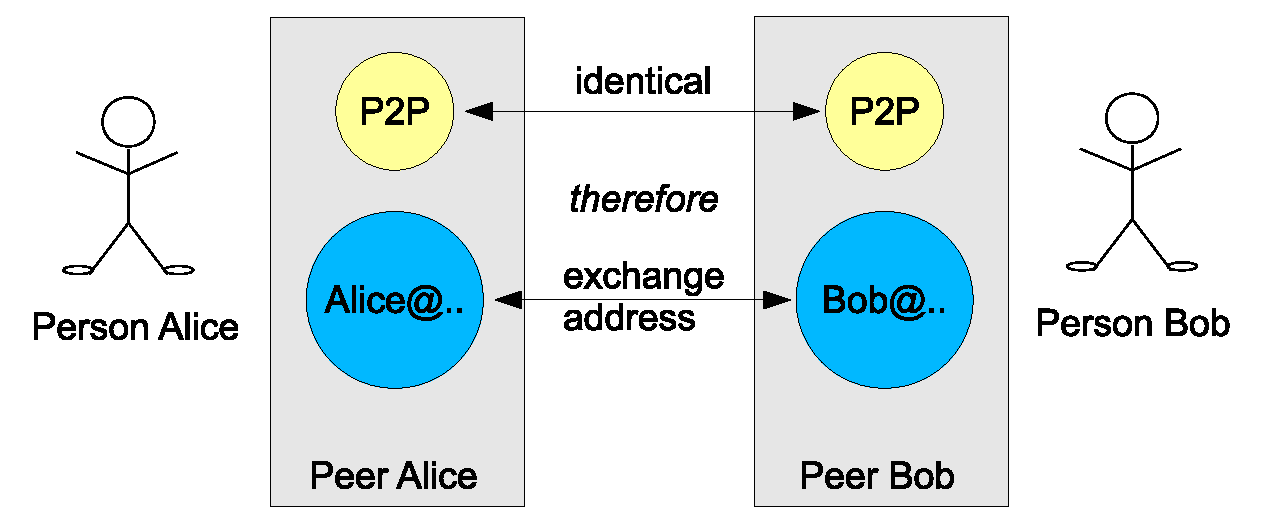
\includegraphics[width=0.60\textwidth]{basisscenario.eps}
\caption{Alice and Bob meet first time}
\label{fig:basisscenario}
\end{figure}

Alice can now send e.g. information about {\it P2P systems} to Bob using e-mail.
They have met in a spontaneous network, learned about their interests and have also learned a more permanent address which allows them to communicate not only in a spontaneous network.

Programming that basic scenario requires a bit more than a dozen lines of code and will be explained in section \ref{sec:knowledgePorts:StandardKP}.

\subsection{Triangle scenario}
We want to expand the base scenario. Clara may enter the scene. She is also interested in {\it P2P systems} and has also just set up her system.

\begin{figure}[t]
\centering
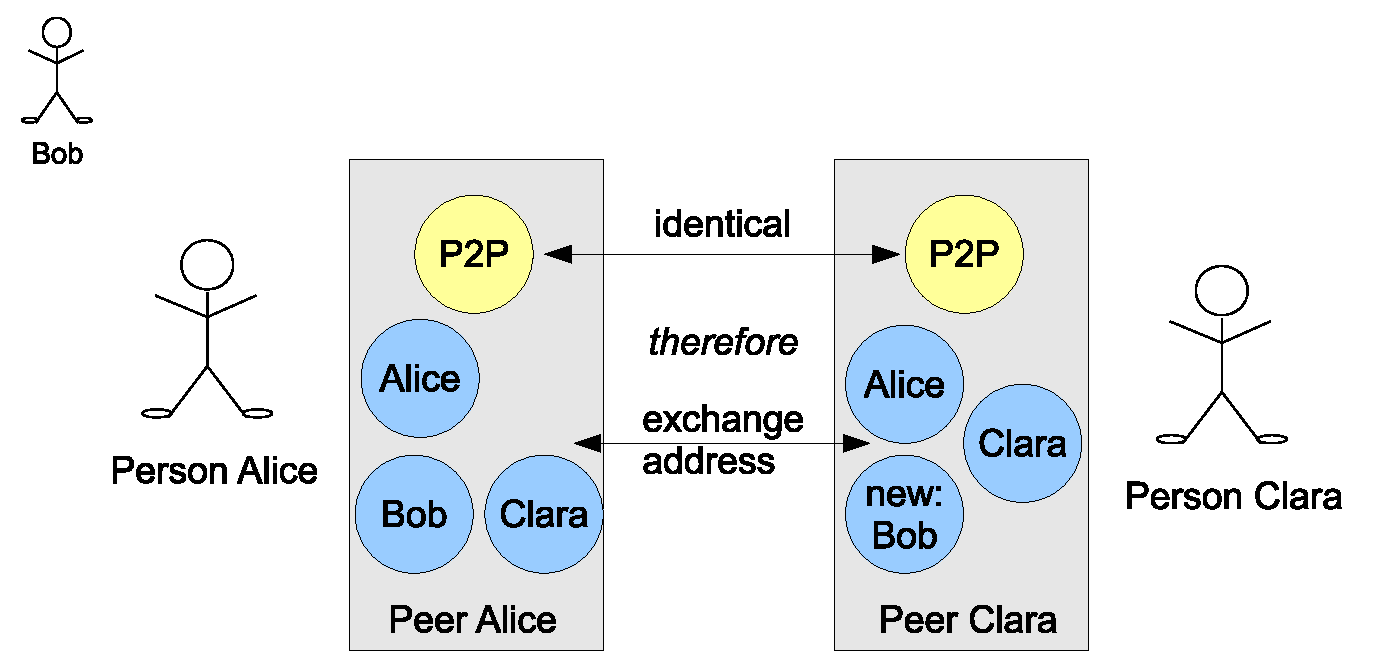
\includegraphics[width=0.60\textwidth]{triangle.eps}
\caption{Alice tell Clara about Bob}
\label{fig:triangle}
\end{figure}

Clara meets her friend Alice. Alice has already met Bob. What happens? First, both perform the base scenario and learn each others interests, addresses and can also exchange information.

Moreover, Alice can\footnote{Can, not must! Any communication behavior can be changed and freely programmed that it fits application needs.} also provide Bobs interest to Clara. In this case, Clara would have {\it met} -- in terms of Shark -- Bob without meeting him personally.

Now, Clara knows Alice and Bob. Alice knows Bob and Clara and Bob just knows Alice. Maybe Clara sends some information to Bob. In this case he would {\it meet} her as well, see figure \ref{fig:triangle}.

\subsection{Hub scenario}
The triangle scenario leads directly to the hub scenario.

Lets introduce a special peer called {\it Hub}. A Hub has also a permanent address. It has no interests by its own but it is willing to receive any interest from other peers.

Let's imagine, that Hub was just set up and imagine that Alice and Bob didn't meet. Alice could expose her interest in {\it P2P systems} to the Hub. Nothing would happen. As the Hub has no interests by its own and no information to deliver.

Bob could also expose his interest to the Hub. The Hub could now check whether there is a matching interest or not. In this example, it would find Alices interest and would send it to Bob. Bob knows Alice now. He can send information to her or expose his interests.

A Hub is meant to help non-mobile peers to meet. It just stores interests and looks for matching interests. It is a kind of matchmaker. It is important to note that a Hub isn't required any longer if peers have finally met, see figure \ref{fig:hub}.

A Hub should be used as a single entity in a real application. There can be an arbitrary number of hubs, though. A Hub should not be considered to be online permanently.

A Hub is actually a special peer with a very limited application logic. There is a predefined class in the Shark framework that can be used in any application. Thus, any peer can become a Hub, see section \ref{sec:hubkp}. Clara was a hub in the previous triangle scenario.

\begin{figure}[t]
\centering
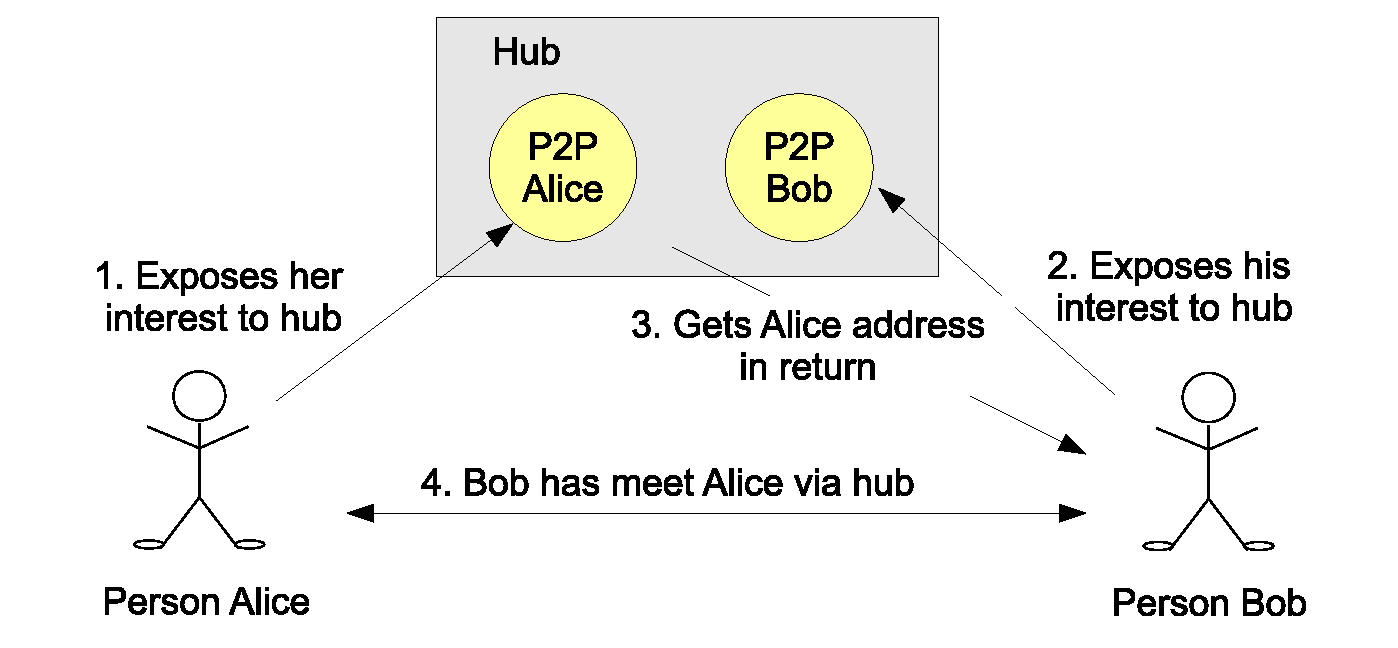
\includegraphics[width=0.60\textwidth]{hub.eps}
\caption{Hub as matchmaker}
\label{fig:hub}
\end{figure}

Of course, interests should be forgotten after a while. The Shark hub implementation allows setting a lifespan for each received interest. The unit is seconds. This underlines the very fact that a hub should not be used as a stable and permanent entity in a fixed infrastructure. Shark applications are P2P applications. As fewer permanent entities exist in a distributed application as more flexible is the overall system.

The Internet is a good example of a reliable system. There are crucial entities but there is no single entity that would switch off the whole network. Web-based applications are different. Just switch off the server (by sabotage, by force (e.g. denial of service attacks), by order of a government, for maintenance, hardware failure or just because also administrators are humans who causes failures) and the whole system is down. A hub shouldn't be used as such a single point of failure and it doesn't has to.

\subsection{Location based scenario}
We can also create a location based service without using GPS and Internet at all. Just take hardware that can establish a spontaneous network and run a peer on it. Let's call this peer {\it Supermarket}. The Supermarket peer can have some product information. It should - of course - be placed into a supermarket.

Let's assume that Alice enters that market. Her peer can establish a connection to the Supermarket peer. Alice should reveal neither her interests nor her address in this scenario. The supermarket on the other hand side should be more verbose and deliver any product information it has.

Alices peer can decide based on her interests which advertisement fits to her interests and which doesn't. That's an automated process. The person Alice wouldn't be aware of any advertisement which is out of her interest.

A supermarket could be replaced by a gallery, a point of (touristic) interest, a fast food shop etc. Such a peer can also be placed near the office door of an elderly professor to submit his lecture notes to interested students who are passing by.
